\documentclass[10pt]{article}
\usepackage[usenames]{color} %used for font color
\usepackage{amssymb} %maths
\usepackage{amsmath} %maths
\usepackage[utf8]{inputenc} %useful to type directly diacritic characters
\usepackage{tikz-cd}
\usepackage{quantikz}
\usetikzlibrary{decorations.markings,decorations.pathmorphing,decorations.pathreplacing}

\definecolor{primary}{RGB}{177,98,78}
\definecolor{secondary}{RGB}{91,132,177}
\definecolor{tertiary}{RGB}{175,195,62}

\begin{document}
\begin{align*}% \tikzset{every picture/.style={/utils/exec={\sffamily}}}
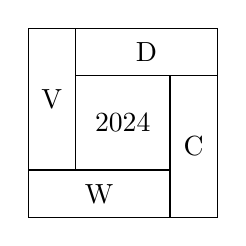
\begin{tikzpicture}[scale=0.6]
\draw (0,1) rectangle (1,4) node[midway]{V};
\draw (1,3) rectangle (4,4) node[midway]{D};
\draw (3,0) rectangle (4,3) node[midway]{C};
\draw (0,0) rectangle (3,1) node[midway]{W};
\node at (2,2) {2024};
\end{tikzpicture}\end{align*}
\end{document}